% ============================================================
%  Presentación Resumen — Metaheurísticas para el LRP
%  Portada + 6 diapositivas de contenido
% ============================================================
\documentclass[aspectratio=169,10pt]{beamer}

\usepackage[T1]{fontenc}
\usepackage[utf8]{inputenc}

\usetheme{Madrid}
\usecolortheme{whale}
\usefonttheme[onlymath]{serif}

\usepackage{amsmath,amssymb}
\usepackage{booktabs}
\usepackage{xcolor}
\usepackage{graphicx}
\usepackage{tikz}
\usetikzlibrary{positioning,shapes.geometric,arrows.meta,calc,fit}
\usepackage{pgfplots}
\pgfplotsset{compat=1.18}
\usepackage{colortbl}

\definecolor{myblue}{RGB}{0,70,127}
\definecolor{mygreen}{RGB}{0,130,0}
\definecolor{myorange}{RGB}{200,100,0}
\definecolor{mygray}{RGB}{140,140,140}

\title[Metaheurísticas para el LRP]{%
  Metaheurísticas para el\\
  \textit{Location Routing Problem}}
\subtitle{ALNS · MA$|$PM}
\author[Lizárraga \& Loayza]{%
  Sebastián Andre Lizárraga Calderón \and
  Johannes Albert Loayza Huamán}
\date{Proyecto Final de Carrera --- 2026}

\setbeamertemplate{navigation symbols}{}
\setbeamertemplate{footline}[frame number]

% ============================================================
\begin{document}

% ── PORTADA ──────────────────────────────────────────────────
\begin{frame}
  \titlepage
  \vspace{-0.8em}
  \begin{center}\small
    Implementación en C++17 de dos metaheurísticas para optimización logística:\\[0.2em]
    \textbf{ALNS} (Adaptive Large Neighborhood Search) \;$+$\;
    \textbf{MA$|$PM} (Memetic Algorithm with Population Management)\\[0.2em]
    validadas sobre benchmarks Prodhon ($n$ = 10--200 clientes)
  \end{center}
\end{frame}

% ════════════════════════════════════════════════════════════
% DIAPOSITIVA 1 — EL PROBLEMA LRP
% ════════════════════════════════════════════════════════════
\begin{frame}{El Problema LRP (Location Routing Problem)}
  \begin{columns}[T,onlytextwidth]
    % ── columna izquierda ──
    \begin{column}{0.36\textwidth}
      {\small\textbf{Tres decisiones simultáneas:}}
      \vspace{0.15em}
      \begin{enumerate}\scriptsize\setlength{\itemsep}{0.15em}
        \item \textbf{Localización:} ¿qué depósitos abrir?\\
              $y_i\!\in\!\{0,1\}$, costo $O_i$, cap.\ $W_i$
        \item \textbf{Asignación:} ¿a qué depósito va cada cliente?\\
              $w_{ij}\!\in\!\{0,1\}$
        \item \textbf{Ruteo:} ¿en qué orden se visitan?\\
              $x_{ij}\!\in\!\{0,1\}$, cap.\ $Q$, costo fijo $F$
      \end{enumerate}
      \vspace{0.25em}
      \rule{\linewidth}{0.4pt}\vspace{0.1em}
      {\small\textbf{Función objetivo:}}\vspace{0.05em}
      {\scriptsize
      \begin{align*}
        \min Z \;=\;&
          \textstyle\sum_{i\in D} O_i\,y_i
          & &\text{(apertura dep.)}\\[-4pt]
          &+\; F\cdot|\mathcal{R}|
          & &\text{(costo fijo)}\\[-4pt]
          &+\; \textstyle\sum_{(i,j)} c_{ij}\,x_{ij}
          & &\text{(distancias)}
      \end{align*}}
      \vspace{-0.2em}
      \rule{\linewidth}{0.4pt}\vspace{0.1em}
      {\scriptsize\textbf{Complejidad:} NP-hard — combina FLP y VRP.
      Las tres decisiones están \textbf{acopladas}: elegir otro depósito
      cambia toda la estructura de rutas.}
    \end{column}
    % ── columna derecha: imagen ──
    \begin{column}{0.62\textwidth}
      \vspace{-0.5em}
      \begin{center}
        \includegraphics[width=\textwidth,height=0.88\textheight,keepaspectratio]%
          {images/LRP_ejem.jpg}
      \end{center}
    \end{column}
  \end{columns}
\end{frame}

% ════════════════════════════════════════════════════════════
% DIAPOSITIVA 2 — ALNS: MECANISMO
% ════════════════════════════════════════════════════════════
\begin{frame}{ALNS --- Mecanismo General}
  \begin{columns}[T,onlytextwidth]
    \begin{column}{0.50\textwidth}
      \begin{center}
      \resizebox{0.88\textwidth}{!}{%
      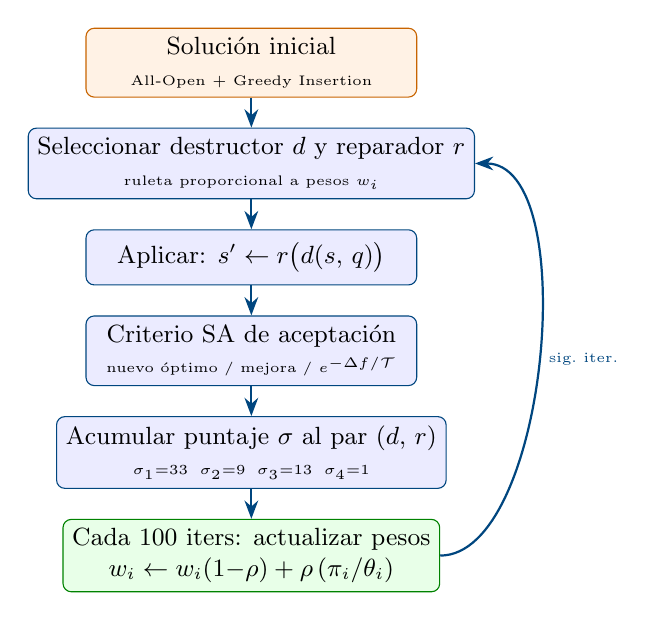
\begin{tikzpicture}[
        b/.style={draw=myblue, fill=blue!8, rounded corners=3pt,
                  minimum width=4.2cm, minimum height=0.70cm,
                  font=\small, align=center},
        g/.style={draw=mygreen, fill=green!9, rounded corners=3pt,
                  minimum width=4.2cm, minimum height=0.70cm,
                  font=\small, align=center},
        o/.style={draw=myorange, fill=orange!10, rounded corners=3pt,
                  minimum width=4.2cm, minimum height=0.70cm,
                  font=\small, align=center},
        arr/.style={-{Stealth}, thick, myblue}
      ]
        \node[o] (s0) {Solución inicial\\
                       {\tiny All-Open + Greedy Insertion}};
        \node[b, below=0.38cm of s0] (s1)
              {Seleccionar destructor $d$ y reparador $r$\\
               {\tiny ruleta proporcional a pesos $w_i$}};
        \node[b, below=0.38cm of s1] (s2)
              {Aplicar: $s' \gets r\bigl(d(s,\,q)\bigr)$};
        \node[b, below=0.38cm of s2] (s3)
              {Criterio SA de aceptación\\
               {\tiny nuevo óptimo / mejora / $e^{-\Delta f/\mathcal{T}}$}};
        \node[b, below=0.38cm of s3] (s4)
              {Acumular puntaje $\sigma$ al par $(d,\,r)$\\
               {\tiny $\sigma_1{=}33$\; $\sigma_2{=}9$\; $\sigma_3{=}13$\; $\sigma_4{=}1$}};
        \node[g, below=0.38cm of s4] (s5)
              {Cada 100 iters: actualizar pesos\\
               $w_i \leftarrow w_i(1{-}\rho)+\rho\,(\pi_i/\theta_i)$};
        \draw[arr] (s0)--(s1); \draw[arr] (s1)--(s2);
        \draw[arr] (s2)--(s3); \draw[arr] (s3)--(s4);
        \draw[arr] (s4)--(s5);
        \draw[arr] (s5.east) to[out=0,in=0,looseness=0.7]
              node[right,font=\tiny]{sig.\ iter.} (s1.east);
      \end{tikzpicture}}
      \end{center}
    \end{column}
    \begin{column}{0.48\textwidth}
      \begin{block}{Simulated Annealing (criterio de aceptación)}\footnotesize
        Solución peor $s'$ aceptada con probabilidad
        $P{=}\exp\!\bigl(-(f(s'){-}f(s))/\mathcal{T}\bigr)$.\\[0.15em]
        Temperatura: $\mathcal{T}{\leftarrow}\alpha\mathcal{T}$
        ($\mathcal{T}_0{=}50\,000$, $\alpha{=}0.998$).\\[0.15em]
        \textit{Alta $\mathcal{T}$: acepta casi todo (explora).
        Baja $\mathcal{T}$: solo acepta mejoras (explota).}
      \end{block}
      \vspace{0.05em}
      \begin{block}{Ruleta Adaptativa (aprendizaje)}\footnotesize
        Cada par destructor+reparador acumula puntaje $\sigma$
        ($\sigma_1{=}33$, $\sigma_2{=}9$, $\sigma_3{=}13$, $\sigma_4{=}1$)
        según la calidad de la solución obtenida.\\[0.15em]
        Cada 100 iters.\ los pesos se actualizan:\\
        $w_i \leftarrow w_i(1{-}\rho)+\rho\,(\pi_i/\theta_i)$,\; $\rho{=}0.1$.\\[0.15em]
        Operadores \textbf{efectivos} $\to$ mayor peso $\to$
        mayor probabilidad de ser elegidos.
      \end{block}
    \end{column}
  \end{columns}
\end{frame}

% ════════════════════════════════════════════════════════════
% DIAPOSITIVA 3 — ALNS: OPERADORES
% ════════════════════════════════════════════════════════════
\begin{frame}{ALNS --- Operadores de Destrucción y Reparación}
  \begin{columns}[T,onlytextwidth]
    \begin{column}{0.50\textwidth}
      {\color{myblue}\textbf{Operadores de Destrucción}}
      {\footnotesize(extraen $q$ clientes a $U$)}
      \vspace{0.2em}
      \begin{itemize}\small\setlength{\itemsep}{0.25em}
        \item \textbf{Random removal:}
              extrae $q$ clientes al azar.
              \textit{Diversificación pura.}
        \item \textbf{Worst removal:}
              extrae los $q$ de mayor costo marginal
              $\Delta_j = c_{aj} + c_{jb} - c_{ab}$.
              \textit{Detecta clientes mal ubicados.}
        \item \textbf{Shaw removal:}
              extrae clientes similares (geográficos) a una semilla.
              \textit{Exploita estructura espacial.}
        \item \textbf{Route removal:}
              elimina una ruta completa al azar.
              \textit{Presiona reducción de flota.}
        \item \textbf{Depot closing:}
              cierra un depósito y libera todos sus clientes.
              \textit{Única acción de localización.}
      \end{itemize}
    \end{column}
    \begin{column}{0.48\textwidth}
      {\color{mygreen}\textbf{Operadores de Reparación}}
      {\footnotesize(reinsertan clientes de $U$)}
      \vspace{0.15em}
      \begin{block}{\textbf{Greedy Insertion} (miope)}\footnotesize
        Evalúa todas las posiciones en todas las rutas e inserta
        donde el costo $\delta = c_{aj}+c_{jb}-c_{ab}$ sea \textbf{mínimo}.
      \end{block}
      \vspace{0.15em}
      \begin{block}{\textbf{Regret-2 Insertion} (previsor)}\footnotesize
        Calcula el \textit{arrepentimiento} de cada cliente:
        $regret(j) = \delta^{(2)}(j) - \delta^{(1)}(j)$.\\[0.1em]
        Inserta primero al de \textbf{mayor} $regret$: el que más
        perdería si espera. \textit{Evita bloquear posiciones críticas.}
      \end{block}
      \vspace{0.15em}
      {\scriptsize\textbf{Nota:} $\delta$ (inserción) y $\Delta$ (remoción)
      usan la misma fórmula $c_{aj}+c_{jb}-c_{ab}$ en sentido opuesto.}
    \end{column}
  \end{columns}
\end{frame}

% ════════════════════════════════════════════════════════════
% DIAPOSITIVA 4 — MA|PM: REPRESENTACIÓN Y DECODIFICACIÓN
% ════════════════════════════════════════════════════════════
\begin{frame}{MA$|$PM --- Representación y Decodificación (Split)}
  \begin{columns}[T,onlytextwidth]
    \begin{column}{0.48\textwidth}
      \begin{block}{Codificación indirecta: el Cromosoma}\small
        En lugar de rutas explícitas, el MA$|$PM usa una representación de dos partes:
        \vspace{0.3em}
        \begin{description}[\textbf{CS}]
          \item[\textbf{DS}] Vector de $m$ enteros:
                $DS[i] > 0 \Rightarrow$ depósito $i$ \textbf{abierto}.
          \item[\textbf{CS}] Permutación de los $n$ clientes
                (\textit{Giant Tour}): un recorrido continuo sin
                indicar depósitos ni rutas.
        \end{description}
      \end{block}
      \vspace{0.2em}
      {\footnotesize\textbf{Ejemplo} con $n=5$, $m=2$, $D_1$ y $D_2$ abiertos:}
      \vspace{0.1em}
      \begin{center}
      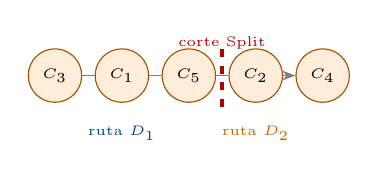
\begin{tikzpicture}[
        nd/.style={circle, draw=myorange!80!black, fill=orange!15,
                   minimum size=0.56cm, font=\tiny}
      ]
        \node[nd] (n0) at (0.00,0) {$C_3$};
        \node[nd] (n1) at (0.85,0) {$C_1$};
        \node[nd] (n2) at (1.70,0) {$C_5$};
        \node[nd] (n3) at (2.55,0) {$C_2$};
        \node[nd] (n4) at (3.40,0) {$C_4$};
        \draw[-{Stealth},gray,thin]
              (n0.east)--(n1.west) (n1.east)--(n2.west)
              (n2.east)--(n3.west) (n3.east)--(n4.west);
        \draw[red!70!black, very thick, dashed] (2.12,-0.40)--(2.12,0.40);
        \node[font=\tiny, myblue,   below=5pt of n1] {ruta $D_1$};
        \node[font=\tiny, myorange, below=5pt of n3] {ruta $D_2$};
        \node[font=\tiny, red!65!black, above=6pt] at (2.12,0) {corte Split};
      \end{tikzpicture}
      \end{center}
      \vspace{0.05em}
      {\scriptsize El Giant Tour no dice nada sobre rutas.
      Eso lo decide el \textbf{Split}.}
    \end{column}
    \begin{column}{0.50\textwidth}
      \begin{block}{\textbf{Algoritmo Split} --- decodificador óptimo}\footnotesize
        Construye un \textbf{DAG auxiliar} de $n{+}1$ nodos
        (posiciones de corte en el CS). Existe un arco $u \to v$
        si los clientes $\pi_{u+1} \ldots \pi_v$ forman una
        ruta factible ($\sum d \le Q$), con peso igual al costo
        de esa ruta desde el depósito óptimo.\\[0.2em]
        El \textbf{camino más corto} $0 \to n$ (Bellman-Ford)
        determina los \textbf{puntos de corte} (partición en rutas)
        y el \textbf{depósito} de cada segmento.
        Complejidad: $\mathcal{O}(n^2 m)$.
      \end{block}
      \vspace{0.2em}
      \begin{exampleblock}{¿Por qué es brillante el Split?}\footnotesize
        El cruce genético opera sobre \textbf{permutaciones de clientes}
        sin preocuparse por factibilidad. El Split convierte cualquier
        Giant Tour en rutas y asignaciones \textbf{óptimas}.
      \end{exampleblock}
    \end{column}
  \end{columns}
\end{frame}

% ════════════════════════════════════════════════════════════
% DIAPOSITIVA 5 — MA|PM: EVOLUCIÓN Y DIVERSIDAD
% ════════════════════════════════════════════════════════════
\begin{frame}{MA$|$PM --- Evolución Poblacional y Gestión de Diversidad}
  \begin{columns}[T,onlytextwidth]
    \begin{column}{0.50\textwidth}
      \begin{block}{Cruce OX (Order Crossover)}\footnotesize
        \textbf{1.} Copiar segmento $[\pi_{k_1}\ldots\pi_{k_2}]$ del Padre 1 al hijo.\\
        \textbf{2.} Completar con clientes del Padre 2 en orden, omitiendo duplicados.\\[0.1em]
        \textit{Preserva el orden relativo, que codifica la estructura espacial.}
      \end{block}
      \vspace{0.2em}
      \begin{block}{Búsqueda Local (fase de educación)}\footnotesize
        Aplicada a cada hijo tras Split (\textit{first-improvement}):
        \begin{itemize}\setlength{\itemsep}{0pt}
          \item \textbf{Relocate:} mover un cliente a otra ruta o depósito.
          \item \textbf{Swap:} intercambiar dos clientes de rutas distintas.
          \item \textbf{2-opt:} invertir segmento intra-ruta (elimina cruces).
        \end{itemize}
        \textit{Cada individuo llega a la población ya ``educado''.}
      \end{block}
    \end{column}
    \begin{column}{0.48\textwidth}
      \begin{block}{PM --- Control de Diversidad (BPD)}\footnotesize
        La \textbf{Broken Pairs Distance} cuenta pares adyacentes distintos
        entre dos soluciones:
        $BPD(A,B) = |\text{pares}(A) \triangle \text{pares}(B)|$.\\[0.1em]
        Un hijo entra si $BPD(hijo,P) \ge \Delta$.
        Demasiados rechazos: $\Delta \leftarrow \max(1,\Delta{-}1)$.\\[0.1em]
        \textit{Evita que la población degenere en clones.}
      \end{block}
      \vspace{0.2em}
      \begin{block}{Flujo del algoritmo}\footnotesize
        \textbf{1.} Inicializar $P$ (Savings + aleatorio)\\
        \textbf{2.} Loop: torneo $\to$ OX $\to$ Split $\to$ LS $\to$ BPD $\to$ insertar\\
        \textbf{3.} Al estancarse: reinsertar élite y refrescar $P$\\
        \textbf{4.} Parar si $NbAcc > MaxNbAcc$
      \end{block}
      \vspace{0.15em}
      {\scriptsize\textbf{Parámetros ($n{=}20$, $m{=}5$):}
       $\mu{=}6$ indiv.,\; $MaxNbAcc{=}250$,\; $\Delta_{max}{=}12$.}
    \end{column}
  \end{columns}
\end{frame}

% ════════════════════════════════════════════════════════════
% DIAPOSITIVA 6 — RESULTADOS Y CONCLUSIONES
% ════════════════════════════════════════════════════════════
\begin{frame}{Resultados Experimentales y Conclusiones}
  \begin{columns}[T,onlytextwidth]
    \begin{column}{0.50\textwidth}
      \textbf{Validación exacta (instancias pequeñas)}
      \vspace{0.25em}
      \begin{center}\footnotesize
      \begin{tabular}{lcccc}
        \toprule
        Instancia & $n$ & $m$ & ALNS & MA$|$PM \\
        \midrule
        coord10-2-1 & 10 & 2
          & \cellcolor{green!20}11\,576
          & \cellcolor{green!20}11\,576 \\
        coord10-2-2 & 10 & 2
          & \cellcolor{green!20}15\,912
          & \cellcolor{green!20}15\,912 \\
        coord12-2-1 & 12 & 2
          & \cellcolor{green!20}15\,123
          & \cellcolor{green!20}15\,123 \\
        \bottomrule
      \end{tabular}
      \end{center}
      {\footnotesize\textit{Gap $= 0\%$ en todos los casos respecto al óptimo exacto
      (Fuerza Bruta). Ambas implementaciones son correctas.}}
      \vspace{0.1em}

      \textbf{Benchmark Prodhon — 30 instancias con BKS}
      \vspace{0.15em}
      \begin{center}\scriptsize
      \begin{tabular}{crrrr}
        \toprule
        & & \multicolumn{2}{c}{Victorias} & \\
        \cmidrule(lr){3-4}
        Escala & \#inst. & ALNS & MA$|$PM & CPU ALNS \\
        \midrule
        $n{=}20$  & 4  & 1 & \textbf{3} & ${<}0.1$s \\
        $n{=}50$  & 8  & 4 & 4          & ${<}0.3$s \\
        $n{=}100$ & 12 & \textbf{11} & 1 & $1$--$3$s \\
        $n{=}200$ & 6  & \textbf{6}  & 0 & $6$--$13$s \\
        \midrule
        \textbf{Total} & \textbf{30} & \textbf{22} & \textbf{8} & --- \\
        \bottomrule
      \end{tabular}
      \end{center}
    \end{column}
    \begin{column}{0.48\textwidth}
      \begin{exampleblock}{MA$|$PM --- instancias Prodhon $n{=}20$}\footnotesize
        Gana 3/4. Split + búsqueda local explotan el espacio en
        profundidad. Para $n{=}50$ es mixto (4--4): ambos compiten.
      \end{exampleblock}
      \vspace{0.1em}
      \begin{alertblock}{ALNS --- instancias grandes ($n \ge 100$)}\footnotesize
        Gana 17/18. MA$|$PM tarda \textbf{100$\times$ más}
        con peores resultados. Única opción práctica a gran escala.
      \end{alertblock}
      \vspace{0.1em}
      \begin{block}{Conclusión}\footnotesize
        \begin{itemize}\setlength{\itemsep}{0pt}
          \item Gap $=0\%$ vs.\ óptimo exacto: \textbf{implementación verificada}.
          \item \textbf{MA$|$PM} gana en $n{=}20$; empate técnico en $n{=}50$.
          \item \textbf{ALNS} domina claramente en $n \ge 100$.
          \item Elección depende del tamaño y tiempo disponible.
        \end{itemize}
      \end{block}
    \end{column}
  \end{columns}
\end{frame}

\end{document}
